\title[概率论]{第四讲: 黎曼积分、{\rm Lebesgue}积分、测度与概率 }
%\author[张鑫{\rm Email: xzhangseu@seu.edu.cn} ]{\large 张 鑫}
\institute[东南大学数学学院]{\large \textrm{Email: xzhangseu@seu.edu.cn} \\ \quad  \\
	\large 东南大学\quad 数学学院\\
	\vspace{0.3cm}
	% \trc{ 公共邮箱: \textrm{zy.prob@qq.com}\\
		%  \hspace{-1.7cm}  密\qquad 码: \textrm{seu!prob}}
}
%\date{\rm \today}
\date{}
{ \setbeamertemplate{footline}{}
	\begin{frame}
		\titlepage
	\end{frame}
}

%\section{黎曼积分与 Lebesgue 积分}
\subsection{黎曼积分}
\begin{frame}{黎曼积分}
	\begin{itemize}[<+-|alert@+>]
		\item 函数 $f:[a,b]\mapsto \mathbb{R}$;
		\item 分割 $\Delta$: $a=x_0<x_1<\cdots<x_n=b$;
		\item 黎曼和:
		\[I(f,\Delta):=\sum_{i=0}^{n-1}f(\xi_i)(x_{i+1}-x_i), \ \mbox{其中} \xi_i\in[x_i,x_{i+1}]; \]
		\item 令$|\Delta|:=\max_{1\leq i\leq n}|x_i-x_{i-1}|$, 则若
		\[\lim_{|\Delta|\rightarrow 0}I(f,\Delta)=\lim_{|\Delta|\rightarrow 0}\sum_{i=0}^{n-1}f(\xi_i)(x_{i+1}-x_i)=L:=\int_a^bf(x)dx,\]
		则称 $L$ 为函数 $f$ 在区间 $[a,b]$ 的积分, 并称函数 $f$ 是黎曼可积的.
	\end{itemize}

\end{frame}
\begin{frame}{黎曼积分示意图}
	\begin{figure}[htbp]
		\centering
		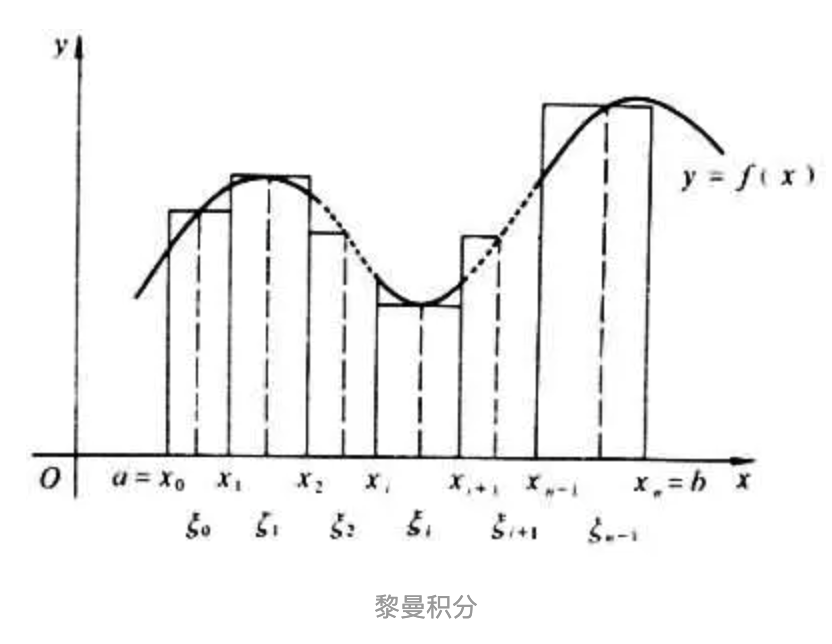
\includegraphics[width=9cm]{Riemanintegral.png}
	\end{figure}
\end{frame}

\begin{frame}{黎曼积分的缺点}
	\begin{itemize}[<+-|alert@+>]
		\item 一些很简单的函数不是黎曼可积的, 如{\rm Dirichlet} 函数:
		\[D(x):=\left\{\begin{array}{ll}
			1, & x \mbox{是有理数},\\
			0, & x \mbox{是无理数}.
		\end{array}\right.\]
		\item 需要一致收敛条件来保证函数积分与极限运算的次序交换, 即若 $f_n(x)$ 一致收敛且黎曼可积, 则
		\[\lim_{n\rightarrow\infty}\int_a^bf_n(x)dx=\int_a^b\lim_{n\rightarrow\infty}f_n(x)dx\]
		\item 黎曼可积函数空间不完备, 即存在黎曼可积函数列 $f_n(x)$ 逐点收敛到函数 $f(x)$, 但 $f(x)$ 不是黎曼可积.
	\end{itemize}
\end{frame}

\begin{frame}{黎曼积分的等价定义(I)}
	\begin{itemize}[<+-|alert@+>]
		\item 考虑函数 $f:[a,b]\mapsto \mathbb{R}$ 及分割 $\Delta$: $a=x_0<x_1<\cdots<x_n=b$, 并令 $|\Delta|:=\max_{1\leq i\leq n}|x_i-x_{i-1}|$ 以及
		\begin{align*}
			M_i(\Delta)&:=\sup_{x_{i-1}\leq x\leq x_i}f(x), \  m_i(\Delta):=\inf_{x_{i-1}\leq x\leq x_i}f(x),\\
			M(\Delta)&:=\sum_{i=0}^{n-1}M_i(x_{i+1}-x_i), \ m(\Delta):=\sum_{i=0}^{n-1}m_i(x_{i+1}-x_i).
		\end{align*}
		\item 上下积分:
		\begin{align*}
			\overline{\int_a^bf(x)dx}&:=\lim_{|\Delta|\rightarrow 0}M(\Delta)=\inf_{\Delta} M(\Delta), \\
			\underline{\int_a^bf(x)dx}&:=\lim_{|\Delta|\rightarrow 0}m(\Delta)=\sup_{\Delta} m(\Delta)
		\end{align*}
		\item  $f(x)$ 黎曼可积当且仅当上下积分相等, 即	$\overline{\int_a^bf(x)dx}=\underline{\int_a^bf(x)dx}$
	\end{itemize}
\end{frame}

\begin{frame}{黎曼积分的等价定义(II)}
	\begin{defi} (分段常值函数或阶梯函数) 函数 $f:[a,b]\mapsto \mathbb{R}$ 称为分段常值函数或阶梯函数, 如果区间 $[a,b]$ 存在一个有限区间分割 $I_1, I_2,\cdots, I_n$ 使得 $f(x)$ 在每个区间上 $I_i$ 上恒为常数 $c_i$, 即
		\[f(x)=\sum_{i=1}^{n}c_i1_{I_i}(x)\]
	\end{defi}
	\pause
	\begin{rmk}
		\begin{itemize}[<+-|alert@+>]
			\item 容易验证, $\sum_{i=1}^nc_i|I_i|$ 与分段常值函数或阶梯函数 $f(x)$ 表达形式中所选择的区间分割无关.%函数
			\item 我们记
			\[p.c.\int_a^bf(x)dx:=\sum_{i=1}^nc_i|I_i|\]
			并将其称为分段常值函数或阶梯函数 $f(x)$ 在 $[a,b]$ 上的积分.
		\end{itemize}
	\end{rmk}
\end{frame}
\begin{frame}{黎曼积分的等价定义(II)}
	\begin{defi} ({\rm Darboux integral} 达布积分) 设函数 $f:[a,b]\mapsto \mathbb{R}$ 为有界函数, 则
		\begin{itemize}[<+-|alert@+>]
			\item 称\[\underline{\int_a^b}f(x)dx:=\sup_{g\leq f,\  g\mbox{为阶梯函数}}p.c.\int_a^bg(x)dx\]
			为函数 $f(x)$ 在 $[a,b]$ 上的达布下积分;%$\underline{\int_a^b}f(x)dx$ 定义为
			\item 称\[\overline{\int_a^b}f(x)dx:=\inf_{h\geq f,\  h\mbox{为阶梯函数}}p.c.\int_a^bh(x)dx\]
			为函数 $f(x)$ 在 $[a,b]$ 上的达布上积分;
			\item 显然, $\underline{\int_a^b}f(x)dx\leq \overline{\int_a^b}f(x)dx$. 如果
			\[\underline{\int_a^b}f(x)dx=\overline{\int_a^b}f(x)dx,\]
			则称函数 $f(x)$ 在 $[a,b]$ 上达布可积.
		\end{itemize}
	\end{defi}

\end{frame}

\begin{frame}{黎曼积分的等价定义(II)}

	\begin{thm}
		设函数 $f:[a,b]\mapsto \mathbb{R}$ 为有界函数, 则函数 $f(x)$ 黎曼可积当且仅当函数 $f(x)$ 达布可积.
	\end{thm}

\end{frame}
\begin{frame}{黎曼积分的本质}

	\begin{itemize}[<+-|alert@+>]
		\item 黎曼积分思想源于古希腊的“穷竭法”.
		\begin{itemize}[<+-|alert@+>]
			\item 求圆的面积: 通过圆外切正 $n$ 边形和内接正 $n$ 边形, 来得到圆面积的上下界, 然后取极限发现上下界都相等, 从而得到圆的面积.
			\item 求函数 $f(x)$ 围成的面积: 把 $f(x)$ 与坐标轴围成的区域通过对定义域 $[a,b]$ 进行有限分割并利用分割小区间上函数 $f(x)$ 的最大最小值构造函数外接与函数内接长方形, 然后取分割的极限得到函数 $f(x)$ 围成的面积.
			\item 黎曼积分整个过程就是: 有限分割--近似求和--取极限.
		\end{itemize}
		\item 对函数\textcolor{cyan}{定义域进行有限区间分割}后近似求和取极限, 适用于连续函数, 即函数在小区间内振荡不明显, 但对然而对于振荡很厉害的函数, 哪怕分割很细, 在很细的区间内振荡依然很厉害(典型的例子是狄利克雷函数).
	\end{itemize}

\end{frame}
\subsection{{\rm Lebesgue} 积分}

\begin{frame}{{\rm Lebesgue} 积分基本思想}

	\begin{itemize}[<+-|alert@+>]
		\item 黎曼积分是对函数的定义域 $[a,b]$ 进行分割, 而{\rm Lebesgue} 积分则是对函数 $f(x)$ 的值域进行分割.
		\item  令 $l<L$ 分别为 $f(x)$ 在区间 $[a,b]$ 上的下确界与上确界, 考虑 $[l,L]$ 的分割 $\Delta_y$:
		\[l=l_0<l_1<l_2<\cdots<l_n=L\]

	\end{itemize}
	\pause
	\begin{figure}[htbp]
		\centering
		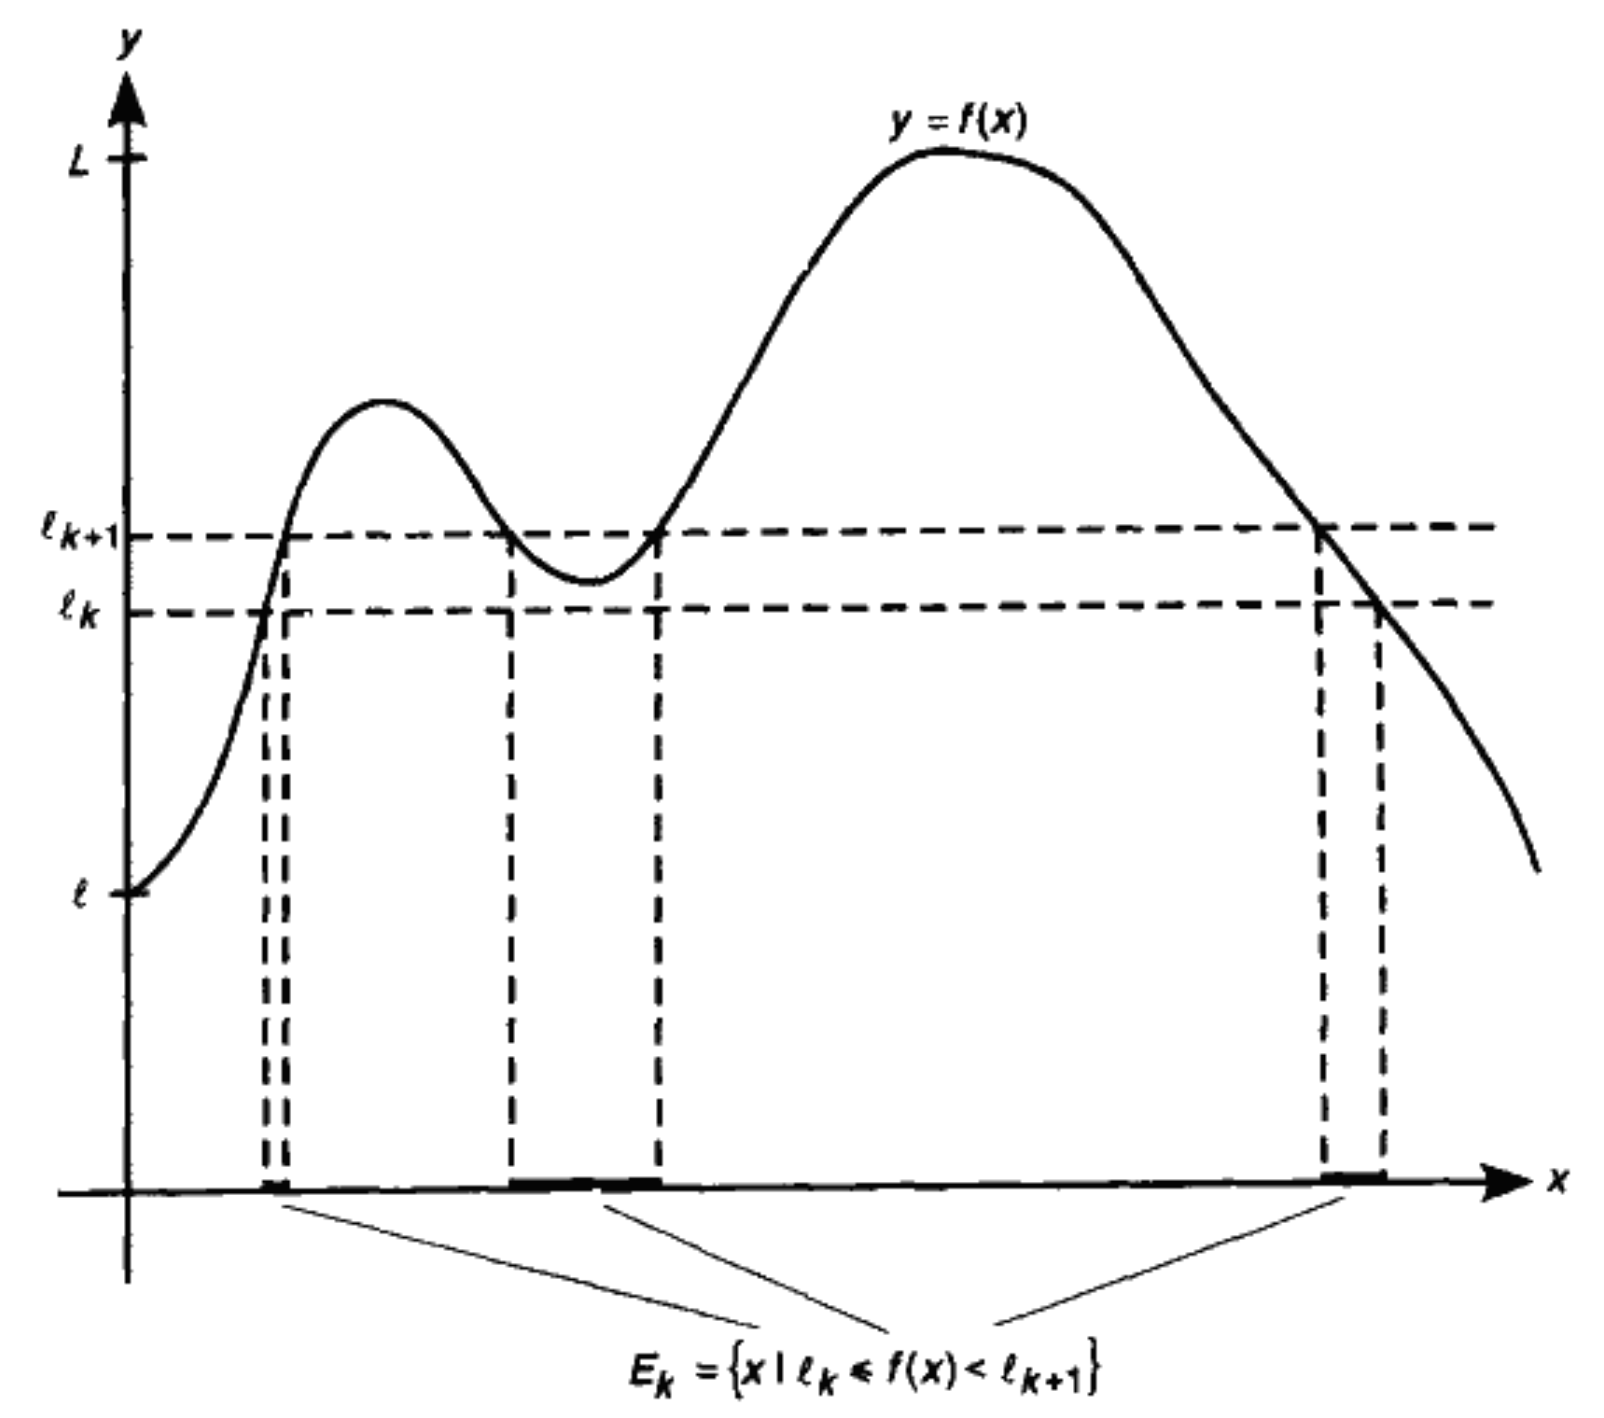
\includegraphics[width=9cm, height=4.8cm]{Lebesgueintegral.png}
	\end{figure}
\end{frame}
\begin{frame}{{\rm Lebesgue} 积分基本思想}

	\begin{itemize}[<+-|alert@+>]
		\item 令
		\begin{align*}
			|\Delta_y|&:=\max_{1\leq k\leq n}|l_k-l_{k-1}|, \\
			E_k&:=\{x:l_k\leq f(x)<l_{k+1}\}, k=0,1,\cdots, n-1,
		\end{align*}
		\item 显然
		\begin{align*}
			\sum_{k=0}^{n-1}l_k1_{E_k}(x)\leq f(x)<\sum_{k=0}^{n-1}l_{k+1}1_{E_k}(x), \forall x\in [a,b].
		\end{align*}
		因此, 相应的积分应保持上述不等关系, 即
		\begin{align*}
			\sum_{k=0}^{n-1}l_k\int_{a}^{b} 1_{E_k}(x)dx\leq \int_{a}^{b}f(x)dx<\sum_{k=0}^{n-1}l_{k+1}\int_{a}^{b}1_{E_k}(x)dx.
		\end{align*}
		\item 类似于黎曼积分的想法, 我们希望当值域分割$|\Delta_y|\to 0$时, 上述左右两端的极限存在且相等.
	\end{itemize}

\end{frame}


\begin{frame}{{\rm Lebesgue} 积分基本思想}

	\begin{itemize}[<+-|alert@+>]

		\item  若对每一个$E_k, k=0, \cdots, n-1$, 示性函数$1_{E_k}(x)$黎曼可积, 且$|\Delta_y|<\epsilon$, 则
		\begin{align*}
			\sum_{k=0}^{n-1}(l_{k+1}-l_k)\int_{a}^{b} 1_{E_k}(x)dx\leq \epsilon \sum_{k=0}^{n-1}\int_{a}^{b}1_{E_k}(x)dx=\epsilon (b-a).
		\end{align*}


		\item  若示性函数$1_{E_k}(x)$不是黎曼可积的,  如何定义:
		\begin{align*}
			m(E_k):=\int_{a}^{b}1_{E_k}(x)dx,
		\end{align*}
		也即集合$E_k$的测度$m(E_k)$如何定义?


		\item 若我们可以定义$m(E_k)$, 则我们可以类似于“黎曼和”一样, 我们构造“勒贝格和”, 用面积已知的一些区域逼近曲线下方的区域:
		\[\int_a^bf(x)dm:=\lim_{|\Delta_y|\rightarrow 0}\Big[\sum_{k=0}^{n-1}l_k\cdot m(E_k)\Big].\]
	\end{itemize}

\end{frame}
\begin{frame}{黎曼积与与{\rm Lebesgue} 积分的直观解释}

	\begin{itemize}[<+-|alert@+>]%微积分的历程 245-246
		\item 想像一位零售商,在一天结束营业时汇总今天的营业收入.
		\begin{itemize}
			\item 黎曼积分法: 从钱箱中依次取出现金累加计算获得总的营业收入;
			\item{\rm Lebesgue} 积分法: 先将钱箱中的现金按面值进行分类, 用面值乘以该面值现金的数量并累加求和获得总的营业收入.
		\end{itemize}
	\end{itemize}

\end{frame}




\subsection{集合的测度}

\begin{frame}
	\frametitle{如何测量集合大小}
	\begin{itemize}[<+-|alert@+>]
		\item  基数或势({\rm Cardinality}): 集合元素的个数;
		\item 称两个集合的基数相等, 如果两个集合之间存在一一映射;
		\item $A=\{2,4,6,\cdots,\}$与$B=\{1,2,3,4,\cdots\}$的基数是相等的;
		\item  基数或势的优缺点:
		\begin{itemize}[<+-|alert@+>]
			\item 在有限集上,基数还是很有用处的;
			\item 但对于无限集情形,这个度量显得过于粗糙,例如,实数集上任意两个区间的基数都是相同的;
		\end{itemize}
		\item 对于连续的集合,我们又有自然的``体积"的概念: \\
		一维空间:长度; 二维空间:面积; 三维空间:传统的体积;


	\end{itemize}
\end{frame}
\begin{frame}{可数集与不可数集}
\begin{itemize}[<+-|alert@+>]
	\item 称集合是可数(countable)的, 如果该集合和自然数集${\mathbf{N}}$的子集之间存在一一映射, 否则称该集合是不可数(uncountable)集.
	\item 可数集包括有限可数集和无穷可数集.
	\item 有限个可数集的并仍然是可数集,可数个可数集的并仍然是可数集.
	\item 两个可数集的笛卡尔积是可数集.
	\item 实数区间 ${(0,1)}$ 是典型的不可数集.\pause

	假设 ${(0,1)}$ 可数, 其元素可以排列为 ${a_{1}, a_{2}, a_{3}, \cdots}$. 注意到 ${(0,1)}$ 中的元素 ${a_{n}}$ 可以表示为
	\[
	a_{n}=0. a_{n}^{(1)} a_{n}^{(2)} a_{n}^{(3)} \cdots=\sum_{k=1}^{\infty} a_{n}^{(k)} 10^{-k}
	\]
	\pause

	构造 ${x=0.x_{1} x_{2} x_{3} \cdots}$, 其中, 对任意的 ${k}$, 取 ${x_{k} \neq a_{k}^{(k)}}$. \pause 显然, $x \neq a_{k}$, $\forall k \in \mathbf{N}$,矛盾.故 ${(0,1)}$ 是不可数集合. 由于
	\[
	f(x)=-\cot (\pi x):(0,1) \rightarrow(-\infty, \infty)
	\]

	是一一映射, 立刻得到 ${\mathbf{R}}$ 也是不可数集. %${\mathbf{R}}$ 是最典型、最重要的不可数集.
\end{itemize}

\end{frame}


\begin{frame}
	\frametitle{集合的测度}
	\begin{itemize}[<+-|alert@+>]
		\item 对于集合大小, 我们希望定义另外的度量标准:测度.
		\begin{itemize}[<+-|alert@+>]
			\item 希望定义一个测度来测量集合的大小,能够处理各种情况,包括有限集、无限集甚至是各种抽象的集合;
			\item 希望在某些特定的情况下,和我们熟知的度量相容:比如区间的长度,区域的面积,空间的体积等度量相容;
			\item 希望具有常见度量的一些性质:可加性.
		\end{itemize}
		\item 如此一来, 设计一个测度就好像变成了制造一把尺子(或者量筒:多维情形).
		\item 尺子有其适用范围:用一个普通米尺来测量地球的半径估计会很有困难,或者用它去测量原子的半径也是不可能的.
		\item 测度的适用范围在测度论里同样重要:在定义一个测度的时候,我们需要同时定义哪些集合是“可测的"({\rm measurable}) -- 也就是可以用这个测度来衡量.
	\end{itemize}
\end{frame}
\subsection{测度的构造}
\begin{frame}
	\frametitle{区间、矩形、基本集及其测度}
	\begin{itemize}[<+-|alert@+>]
		\item 区间 $I\subset\mathbb{R}$ : $[a,b],\  [a,b),\  (a,b), \cdots$;
		%		\item 矩形 $B\subset\mathbb{R}^d$: $[a,b]\times[c,d],\  [a,b]\times [c,d), \cdots$;
		%		\item 方体 $B\subset\mathbb{R}^d$:
		\item 矩形 $B\subset\mathbb{R}^d$: $B:=I_1\times \cdots\times I_d$, 其中$I_i$ 为区间;
		\item 矩形的测度: $|B|:=|I_1|\times|I_2|\times\cdots\times|I_d|$
		\item 基本集 $E\subset\mathbb{R}^d$: 能够表示为有限个矩形的并的集合;
		\begin{itemize}[<+-|alert@+>]
			\item 更进一步, 可以证明基本集一定可以表示为有限个不相交矩形的并, 即
			\[E=\cup_{i=1}^kB_i, \mbox{其中} B_i, i=1,\cdots, k, \mbox{为矩形且互不相交};\]
			\item 我们将 $m(E):=|B_1|+|B_2|+\cdots+|B_k|$ 称为基本集 $E$ 的基本测度.
		\end{itemize}
	\end{itemize}
\end{frame}
\begin{frame}
	\frametitle{约当测度({\rm Jordan Measure})}
	\begin{defi}
		(约当测度) 令 $E$ 为 $\mathbb{R}^d$ 的有界子集.
		\begin{itemize}
			\item 称
			\[m_{*,J}(E):=\sup_{A\subset E, A\mbox{为基本集}}m(A)\]
			为约当内测度;
			\item 称
			\[m^{*,J}(E):=\inf_{A\supset E, A\mbox{为基本集}}m(A)\]
			为约当外测度;
			\item 称 $E$ 为约当可测的, 如果 $m_{*,J}(E)=m^{*,J}(E)$. 此时称 $m(E):=m_{*,J}(E)=m^{*,J}(E)$ 为集合 $E$ 的约当测度.
		\end{itemize}
	\end{defi}
\end{frame}
\begin{frame}
	\frametitle{约当测度的优缺点}
	设 $E,\  F\subset\mathbb{R}^d$ 为约当可测集, 则
	\begin{itemize}[<+-|alert@+>]
		\item $E\cup F,\  E\cap F,\  E\backslash F,\  E\Delta F$ 均为约当可测集;
		\item 非负性: $m(E)\geq 0$;
		\item 有限可加性: 如果 $E, F$ 不相交, 则 $m(E\cup F)=m(E)+m(F)$;
		\item 平称不变性: $m(x+E)=m(E)$;
		\item $E_i, i=1,2,\cdots$ 约当可测, 但 $\cup_{i=1}^\infty E_i, \  \cap_{i=1}^\infty E_i$ 不一定约当可测
	\end{itemize}
\end{frame}

\begin{frame}{{\rm Riemann }积分与{\rm Jordan} 测度之间的联系}
\begin{thm}({\rm Riemann }积分与{\rm Jordan} 测度之间的联系)
	\begin{itemize}
		\item  如果 $E$ 是区间 $[a,b]$ 上的{\rm Jordan} 可测集, 则示性函数
		\begin{align*}
			1_{E}(x):=\left\{\begin{array}{ll}
				1, & x\in E \\ 0, & x\notin E \end{array}\right.
		\end{align*}
		是{\rm Riemann } 可积的且 $\int_{a}^b{1}_{E}(x) \, dx=m(E)$.
		\item  设 $[a,b]$ 为一区间, $f:[a,b]\rightarrow \mathbb{R}$ 为一有界函数, 则 $f$ 是{\rm Riemann }可积当且仅当
		\begin{align}
			E_+ &:=\{(x,t):x\in[a,b], 0\leq f(x)\leq t\}\\ E_-&:=\{(x,t):x\in[a,b], f(x)\leq t\leq 0\}
		\end{align}
		在 $\mathbb{R}^2$ 上是{\rm Jordan} 可测的, 且有
		$$\int_{a}^b f(x)  \, dx=m_{2}(E_{+})-m_{2}(E_{-}) $$
		此处的 $m_{2}$ 表示二维{\rm Jordan}  测度.
	\end{itemize}

\end{thm}
\end{frame}




\begin{frame}
	\frametitle{{\rm Lebesgue}测度}

	\begin{itemize}[<+-|alert@+>]
		\item{\rm Lebesgue}外测度$m^*(E)$:
		\[m^*(E):=\inf_{\cup_{i=1}^\infty B_i\supset E, B_i, i\geq 1, \mbox{为矩形}}\sum_{i=1}^\infty |B_i|\]
		\item 显然, $m^*(E)\leq m^{*,J}(E)$, 且存在$E\subset\mathbb{R}^d$使得不等号严格成立;
		\item{\rm Lebesgue}可测集的卡拉西奥多里({\rm Carath{\'e}odory})准则:\pause
		\vspace{0.4cm}

		称$E\subset\mathbb{R}^d$为{\rm Lebesgue}可测集, 如果对任意的$S\subset\mathbb{R}^d$均有
		\[m^*(S)=m^*(S\cap E)+m^*(S\backslash E),\]
		并称$m(E):=m^*(E)$为集合$E$的\textcolor{cyan}{{\rm Lebesgue}测度}.
	\end{itemize}
\end{frame}

\begin{frame}
	\frametitle{{\rm Lebesgue}可测集的代数结构}
	\begin{defi}\textcolor{cyan}{(事件或集合的{\rm Borel} 运算)}
		我们将对所给出的一些事件或集合所作的各种 (有限次或可列次) 取余、取交和取并运算以及它们的混合运算都称为 \textcolor{cyan}{事件或集合的{\rm Borel} 运算}。
	\end{defi}
\vspace{0.3cm}

	\pause
	\begin{defi}\textcolor{cyan}{($\sigma-$代数)} 设$\mathcal{F}$为$\mathbb{R}^d$的某些子集构成的集合类, 称$\mathcal{F}$为 $\mathbb{R}^d$上的$\sigma$-代数, 如果
		\begin{enumerate}[<+-|alert@+>][(1)]
			\item $\emptyset\in \mathcal{F}$;
			\item 若$A\in \mathcal{F}$, 则 $\overline{A}:=\mathbb{R}^d-A\in \mathcal{F}$;
			\item 若$A_i\in \mathcal{F}, i=1, 2,\cdots,$, 则$\cup_{i=1}^{\infty}A_i\in \mathcal{F}$.
		\end{enumerate}
	\end{defi}

	\vspace{0.3cm}
\pause
\begin{prop}
  在$\mathbb{R}^d$上的Lebesgue可测集具有以下性质:
  \begin{itemize}[<+-|alert@+>]
	\item 若$E,\  F\subset\mathbb{R}^d$ {\rm Lebesgue}可测, 则$E\cup F,\  E\cap F,\  E\backslash F,\  E\Delta F$ 均{\rm Lebesgue}可测;
	\item 若$E_i, i\geq 1$,{\rm Lebesgue}可测, 则$\cup_{i=1}^\infty E_i, \  \cap_{i=1}^\infty E_i$ 也{\rm Lebesgue}可测.
\end{itemize}
\end{prop}


\end{frame}


\begin{frame}
	\frametitle{{\rm Lebesgue}测度的性质}


	\begin{itemize}[<+-|alert@+>]
		\item 非负性: $m(E)\geq 0$;
		\item $m(\emptyset)=0$;
		\item 可列可加性: 如果 $E_i, i\geq 1 $ 互不相交且{\rm Lebesgue}可测, 则 \[m(\cup_{i=1}^\infty E_i)=\sum_{i=1}^\infty m(E_i);\]
		\item 平移不变性: $m(x+E)=m(E)$;
		\item 存在$F\subset\mathbb{R}^d$不{\rm Lebesgue}可测.

	\end{itemize}
\end{frame}









\begin{frame}
	\frametitle{不可测集}
	\textcolor{cyan}{巴拿赫-塔斯基分球悖论({\rm Banach-Tarski Paradox})}

	\qquad   将一个三维的半径为 $1$ 的实心球用某种巧妙方法分成五等分(五等分的意思是,把其中一份旋转平移后可以和另外一份重合), 然后把这五个分块旋转平移后,可以组合成两个半径为 $1$ 的实心球.

	\begin{figure}[htbp]
		\centering
		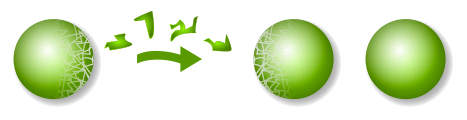
\includegraphics[width=9cm]{fenqiu.jpg}
	\end{figure}
	\pause
	\textcolor{cyan}{选择公理({\rm Axiom of Choice})}:  任意一组(可能有不可数无限个)非空集合,我们都可以从每个集合挑出一个元素.
\end{frame}

\begin{frame}
	\frametitle{巴拿赫-塔斯基分球悖论的启示}
	\begin{itemize}[<+-|alert@+>]
		\item  在$\Omega=\mathbb{R}^3$时, 无法构造出一个测度既与常见的体积度量相容且具有平移不变性,又可以度量$\mathbb{R}^3$的任一子集;
		\item 类似的, 在$\Omega=\mathbb{R}$ 时,同样无法构造出一个测度既与常见的长度度量相容且具有平移不变性,又可以度量$\mathbb{R}$的任一子集; (\tc{不可测集构造详见教材第33-34页2.4节``不可测集".})
		\item 因此,对于可测空间$(\Omega,\mathcal{F})$中的$\mathcal{F}$通常为$\Omega$的某些子集构成的$\sigma$代数,而不一定是$\Omega$的所有子集构成的集类.

	\end{itemize}
\end{frame}

\begin{frame}
	\frametitle{ 由{\rm Lebesgue}测度到一般抽象测度}
	\begin{itemize}[<+-|alert@+>]
		\item 要度量集合元素的全体: $\Omega$
		\item 测度的适用范围(定义域): $\mathcal{F}:=\{A\subset \Omega:A\mbox{可测}\}$, 通常要求$\mathcal{F}$为$\sigma$-代数
		\item 通常称$(\Omega, \mathcal{F})$为可测空间
		\item 测度的定义: 称定义在$\mathcal{F}$的集函数$\mu(\cdot)$为测度, 如果
		\begin{enumerate}[<+-|alert@+>][(1)]
			\item $\mu(A)\ge 0, \forall A\in \mathcal{F}$;
			\item $\mu(\emptyset)=0$;
			\item $\mu$具有可列可加性: 若$A=\cup_{i=1}^{\infty}A_i$, 其中$A, A_i\in \mathcal{F}$,  且$i\neq j$时, $A_i\cap A_j=\emptyset$,  则
			\begin{eqnarray*}
				\mu(\cup_{i=1}^{\infty}A_i)=\sum_{i=1}^{\infty}\mu(A_i)
			\end{eqnarray*}

		\end{enumerate}
		\item  称$(\Omega,\mathcal{F},\mu)$为测度空间.
	\end{itemize}

\end{frame}

\subsection{概率与测度}


% \begin{frame}
% 	\frametitle{事件域或$\sigma$-代数}

% 	\begin{defi}\textcolor{cyan}{($\sigma-$代数)} 设$\mathcal{F}$为$\Omega$的某些子集构成的集合类, 称$\mathcal{F}$为 $\Omega$上的$\sigma$-代数(或事件域), 如果
% 		\begin{enumerate}[<+-|alert@+>][(1)]
% 			\item $\Omega\in \mathcal{F}$;
% 			\item 若$A\in \mathcal{F}$, 则 $\overline{A}:=\Omega-A\in \mathcal{F}$;
% 			\item 若$A_i\in \mathcal{F}, i=1, 2,\cdots,$, 则$\cup_{i=1}^{\infty}A_i\in \mathcal{F}$.
% 		\end{enumerate}
% 	\end{defi}

% \end{frame}

% \begin{frame}
% 	\frametitle{常见的事件域}
% 	\begin{itemize}[<+-|alert@+>]
% 		\item 若$\Omega=\{\omega_1,\omega_2\}$: 记$A=\{\omega_1\}, \overline{A}=\{\omega_2\}$, 则 $\mathcal{F}:=\{\emptyset, A,\overline{A}, \Omega\}$为事件域;
% 		\item  若$\Omega=\{\omega_1,\omega_2,\cdots,\omega_n\}$: 则 $\mathcal{F}:=\{A:A\subset \Omega\}$为事件域;
% 		\item 若$\Omega=(-\infty, +\infty)$: 记$\mathcal{P}=\{(-\infty, x):-\infty <x<+\infty\}$, 则 $\mathcal{F}=\mathcal{B}(\mathbb{R}):=\sigma(\mathcal{P})$为事件域.
% 	\end{itemize}
% \end{frame}





\begin{frame}
	\frametitle{概率与测度}
	\begin{itemize}[<+-|alert@+>]
		\item \textcolor{red}{$\Omega$:}  \textcolor{cyan}{概率论中的样本空间对应于测度中要度量的集合所包含元素的全体}
		\item \textcolor{red}{$\mathcal{F}$:} 事件域, 即某些随机事件组成的集合, 通常要求其为$\sigma$-代数;
		\begin{itemize}
			\item 注意到随机事件是随机试验中我们所关心的可能出现的结果, 它由一个或若干个基本事件组成, 因此事件是样本空间的子集, 从而事件域为样本空间的某些子集构成的集合;
			\item \textcolor{cyan}{概率论中的事件域对应于测度中要度量的集合全体即可测集的概念}
		\end{itemize}
		\item \textcolor{red}{$(\Omega,\mathcal{F})$:}可测空间
	\end{itemize}

\end{frame}


\begin{frame}
	\frametitle{概率的公理化定义}

	\begin{defi}\textcolor{cyan}{(概率的公理化定义)} 设$\Omega$为样本空间, $\mathcal{F}$为$\Omega$的某些子集组成的$\sigma$-代数(事件域), 若定义在$\mathcal{F}$上的集函数$P(\cdot)$满足
		\begin{enumerate}[<+-|alert@+>][(1)]
			\item 非负性: $P(A)\geq 0$;
			\item 正则性: $P(\Omega)=1\textcolor{red}{\Rightarrow P(\emptyset)=0 (\mbox{结合可列可加性})}$;
			\item 可列可加性: 若$A_i,i=1,2,\cdots$ 互不相交, 则
			\[P(\cup_{i=1}^\infty A_i)=\sum_{i=1}^\infty P(A_i).\]
		\end{enumerate}
		\pause
		\vspace{-0.5cm}则称$P$为$(\Omega,\mathcal{F})$上的概率测度,简称概率,称$(\Omega,\mathcal{F},P)$为概率空间.
	\end{defi}
\end{frame}

\begin{frame}
	\frametitle{关于概率的几个注记}
	% \vspace{-0.3cm}
	\begin{itemize}[<+-|alert@+>]
		\item 从概率的定义可以看出, 概率是全集度量为 $1$ 的测度;
		\item \tc{概率与我们熟知的度量(长度,面积,体积,质量)相比,本质上没有太大的区别},只不过概率是用来衡量随机事件发生可能性大小的一种度量, 其在全集上的度量为 $1$;
		\item 同一随机试验得到的可测空间$(\Omega,\mathcal{F})$, 可定义不同的概率.
		\begin{itemize}[<+-|alert@+>]
			\item 对于抛一枚硬币这一随机试验,
			\begin{eqnarray*}
				\Omega=\{\mbox{正,反}\}, \mbox{ 选取} \mathcal{F}=\{\emptyset, \{\mbox{正}\}, \{\mbox{反}\}, \Omega\};
			\end{eqnarray*}
			\item 我们可以构造概率$P_1(\cdot)$:
			\[P_1(\emptyset)=0, P_1(\{\mbox{正}\})=1/2,  P_1(\{\mbox{反}\})=1/2,  P_1(\Omega)=1;\]
			\item 也可以构造概率$P_2(\cdot)$: 其中$p+q=1$,
			\[P_2(\emptyset)=0, P_2(\{\mbox{正}\})=p,  P_2(\{\mbox{反}\})=q,  P_1(\Omega)=1.\]
		\end{itemize}

	\end{itemize}
\end{frame}

